\section{Study}
\label{sec:study}

To understand how programmers use regular expressions in Python projects, we scraped \DTLfetch{data}{key}{nProjScanned}{value} Python projects from GitHub, and recorded regex usages for analysis as described in Section~\ref{study:corpus}.
Throughout the rest of this paper, we  employ the following terminology:

\noindent \textbf{Utilization}: A \emph{utilization} occurs whenever a developer uses a regex engine in a project.  Within a particular file in a project, a \emph{utilization} is composed of a function, a pattern and 0 or more flags.  Figure~\ref{fig:exampleUsage} presents an example of one regex \emph{utilization}, with key components labeled. The function called from the {\tt re} module is {\tt re.compile} does \todo{describe this module}, the pattern observed (i.e., a regex string) is {\tt `(0 $\mid$-?[1-9][0-9]*)\$'} represents strings with \todo{briefly describe the regex}, and the flag allows string matching over multiple lines.
Thought of another way, a regular expression  utilization is one single invocation of the {\tt re} library in a project.

\begin{figure}[htb]
\centering
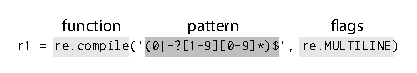
\includegraphics[width=\columnwidth]{../illustrations/exampleUsage.eps}
\caption{example of one regex utilization}
\label{fig:exampleUsage}
\end{figure}



\noindent \textbf{Pattern}: A \emph{pattern} is an ordered series of regular expression language feature tokens that can be used to find match start and end indices within an input string.  Notice that because the vast majority of regex features are shared across most all-purpose languages, a Python {pattern} will (almost always) behave the same when used in Java, C\#, Javascript, Ruby, etc, whereas a {utilization} is not universal in the same way (would not compile in other languages).

In this work, we primarily focus on patterns since these represent \todo{explain why patterns}. 

\subsection{Research Questions}
Our overall research goal is to understand how regular expressions and regular expression features are used in practice. We aim to answer the following research questions:

\textbf{RQ1:} How  is the {\tt re} module used in Python projects?

To address this research question, we measure how often any calls are made to the {\tt re} module per file and per project in Python projects.

Furthermore, we measure the frequency of usage for calls to the 8 functions of the {\tt re} module ({\tt re.compile}, {\tt re.search}, {\tt re.match}, {\tt re.split}, {\tt re.findall}, {\tt re.finditer}, {\tt re.sub} and {\tt re.subn}) in Python projects scraped from GitHub.

We also measure usage of the 8 flags ({\tt re.DEFAULT}, {\tt re.IGNORECASE}, {\tt re.LOCALE}, {\tt re.MULTILINE}, {\tt re.DOTALL}, {\tt re.UNICODE}, {\tt re.VERBOSE} and {\tt re.DEBUG}) of the {\tt re} module.

Further, to provide context as to the overlap among regular expression strings used in Python, we explore the most common regex {patterns} across all utlizations.

\textbf{RQ2:} Which regular expression language features are most commonly used in python?

We consider regex language features to be tokens that specify the matching behavior of a regex pattern, for example,  the {\tt +} in {\tt ab+}.  All studied features are listed and described in Section~\ref{study:corpus} with examples.

To measure feature usage, we parse Python regular expression patterns using Bart Kiers' PCRE parser\todo{add footnote or citation}, as described in Section~\ref{study:corpus}.  We then count the number of usages of each feature per project, per file and as a percent of all distinct regular expression patterns.

\textbf{RQ3:} What is the impact of \emph{not} supporting various regular expression features on tool designers and users?
%\textbf{RQ3:} What is the impact of \emph{not} supporting various regex features on tool designers and users?

To address, this question, we use semantic analysis to illustrate the impact of missing features on a tool's applicability by identifying what each feature (or group of features) is commonly used for.

At a high level, our semantic analysis clusters regular expressions by their behavioral similarity. Behavioral similarity is determined by a pairwise comparison among all patterns. Within each pair, a set of strings is generated for each regular expression and then tested against the other. The average percentage of matching regular expressions creates the similarity level. 

\todo{Finish this example}
For example, consider the following two regular expressions, denoted A and B for reference. 

\begin{verbatim}
state regex A
state regex B
\end{verbatim}

For each regex, the following strings are generated:

\begin{tabular}{l | l} 
A & B \\ \hline
s1 & s2 \\
s3 & s4 \\ 
\end{tabular}

Each string in the A column matches regex A, and each string in the B column matches regex B. When testing the strings in B against regex A, X/5 = 0.Y\% match. When testing the strings in the A column against regex B, Z/5 = 0.W\% match. Thus, the similarity between these two regular expressions is 0.U\%. 

Semantic analysis is accomplished by first establishing a similarity matrix between regexes. These strings are generated by Rex.  Then clusters of regexes with similar behavior are discovered using Markov Clustering\footnote{\url{http://micans.org/mcl/}}.  These clusters are used to interpret what a feature is used for.

We chose Rex to build matching strings because it supports the most features of any String-generation tool.  We chose the mcl clustering tool because it offers a fast and tunable way to cluster items by similarity (without knowing the number of clusters in advance).

\todo{Is this still the case?}
Since our semantic analysis is based on Rex, this semantic analysis cannot be applied to all features studied.  For these unsupported features, we use 6 string similarity metrics (Jaro-Winkler, Levenshtein, Longest Common Substring, Sift3, Jaccard and Cosine) to build similarity matrices.  As before, these matrices are used to find clusters of regexes, which are used to interpret what a feature is used for.




\subsection{Building the Corpus}
\label{study:corpus}
Github is a popular project hosting site containing over 100,000 Python projects.
We used the GitHub api to page through all repositories, cloning projects that contain Python code.

For each project, we used Astroid\footnote{\url{https://bitbucket.org/logilab/astroid}} to build the AST of each Python file and find \emph{utilizations} of Python's {\tt re} module.

Using git, each project was scanned at 20 evenly-spaced commits (or all commits if there were less than 20) in its history.
Within one project, we define a duplicate \emph{utilization} as a \emph{utilization} having the same function, pattern and flags within the same file (same relative path).  We ignored duplicate \emph{utilizations} to protect against over-counting the same \emph{utilization} as we rewind the project through its history.  We observed and recorded \DTLfetch{data}{key}{nUsages}{value} non-duplicate regex \emph{utilizations} in \DTLfetch{data}{key}{nProjScanned}{value} projects.

\subsection{Selecting Patterns}
Because the focus of this study is regex features,  analysis focuses on the patterns found, so we ignored the \DTLfetch{data}{key}{percentBadFlags}{value}\%  of \emph{utilizations} using flags that can alter regex behavior.  An additional \DTLfetch{data}{key}{percentInvalidPattern}{value}\% of \emph{utilizations} contained patterns that could not be compiled because the pattern was non-static (used some runtime variable), or because of other unknown parsing failures.

The remaining \DTLfetch{data}{key}{percentCleanUsages}{value}\% (\DTLfetch{data}{key}{nCleanUsages}{value}) \emph{utilizations} were collapsed into \DTLfetch{data}{key}{nDistinctPatterns}{value} distinct pattern strings.  The resulting set of patten strings were parsed using an antlr-based, open source PCRE parser released by Bart Kiers\footnote{\url{https://github.com/bkiers/pcre-parser}}.  This parser was unable to support \DTLfetch{data}{key}{percentUnicode}{value}\% (\DTLfetch{data}{key}{N_UNICODE}{value}) of the patterns due to unsupported unicode characters.  Another \DTLfetch{data}{key}{percentAlien}{value}\% (\DTLfetch{data}{key}{N_ALIEN}{value}) of the patterns used regex features that we have chosen to exclude in this study\footnote{\url{www.details.#thistopic}}.  The \DTLfetch{data}{key}{nCorpus}{value} distinct pattern strings that remain were each assigned a weight value equal to the number of distinct projects the pattern appeared in.  We will refer to this set of weighted, distinct pattern strings as the \emph{corpus}.

\subsection{Analyzing Features}
\label{study:features}

\todo{revise this subsection}
After picking four large regex research projects, the big table with the features was created in order to decide which unsupported features are used most often.
Our semantic analysis is dependent on the use of Rex to generate strings so we can identify semantically related clusters. For three common features unsupported by Rex, we rely on syntactic analysis to determine similarity among regular expressions containing those features. For those features supported by Rex, we cluster the regular expressions based on semantic diversity.

\subsubsection{Syntactic Diversity}
For the negative perspective, we picked three features: LZY, NCG, WNW that are unsupported by Rex and other projects.  For each of these features, we created a subset of the \emph{collection} where all the patterns contain that feature.  Then we used syntactic analysis...to create a similarity matrix.  We then used markov clustering [X] (MCL) to find clusters in the subset.  We used these clusters to assist our manual search for some common use cases for the unsupported feature.

Markov clustering can be tuned using many parameters, including inflation and filtering out all but the top-k edges for each node.  After exploring the quality of the clusters using various tuning parameter combinations\footnote{\url{www.details.#thistopic}}, the best clusters were found using an inflation value of 1.8 and k=83.

Note that the filteredCorpus is of size 9727, and at least one pattern from the fc can be found in 1375 of the original 3900 or whatever.  Most patterns do not belong in a cluster (for example a very specific pattern like \verb!<title>[^<]*Revision \d+:!), so after clustering is done only 2727 patterns are included, and only 999 projects have any of these patterns in them.


\subsubsection{Semantic Diversity}
For the positive perspective, we created another subset of patterns (XYZ patterns) where Rex was able to generate strings that the pattern matched.  We then created a similarity graph with weighted, undirected edges as shown in Figure~\ref{fig:similarityConstruction}.

\begin{figure}
\begin{description}
\setlength{\parskip}{0pt} % block paragraphs
\setlength{\itemindent}{0in}
\item for each row i:
\setlength{\itemindent}{0.2in}
\item obtain set of Rex-generated strings Ri from pattern at index i
\item sRi = size of Ri
\item for each col j:
\setlength{\itemindent}{0.4in}
\item Nij = number of strings in Ri matched by pattern at index j
\item M[i][j] = Nij/sRi
\setlength{\itemindent}{0in}
\item G = empty graph
\item for each row i:
\setlength{\itemindent}{0.2in}
\item for each col j:
\setlength{\itemindent}{0.4in}
\item SIMij = (M[i][j]+M[j][i])/2
\item if SIMij > 0.75:
\setlength{\itemindent}{0.6in}
\item add edge (i,j)=SIMij to G
\setlength{\itemindent}{0in}
\setlength{\parskip}{10pt} % block paragraphs
\end{description}
\caption{Constructing Similarity Graph \label{fig:similarityConstruction} \todo{replace this algorithm with a textual description}}
\end{figure}

Again we used MCL to find clusters that aided a manual search for use cases strongly associated with particular features.











